\documentclass[12pt]{article}


\topmargin 0pt
\advance \topmargin by -\headheight
\advance \topmargin by -\headsep
\textheight 8.9in
\oddsidemargin 0pt
\evensidemargin \oddsidemargin
\marginparwidth 0.5in
\textwidth 6.5in

\parindent 0in
\parskip 1.5ex
%\renewcommand{\baselinestretch}{1.25}

\usepackage{xr-hyper}
\def\renewtheorem{}

% Note: this has been tested using MiKTeX 2.9. If you are getting errors, update your packages.
% LTeX: enabled=false

%%% Packages %%%
%\usepackage{setspace} % Double spaces document. Footnotes,
% figures, and tables will still be single spaced, however.
%\doublespacing
%\singlespacing
%\onehalfspacing
% \setstretch{1.5} % set double spacing to 1.5 or anything else.


\usepackage[T1]{fontenc}
\usepackage[utf8]{inputenc}
\usepackage{mathtools}

\providecommand{\hmmax}{0}
\providecommand{\bmmax}{0}
\usepackage{amssymb,mathrsfs}% Typical maths resource packages
\usepackage{amsthm}
\usepackage{bm}
\usepackage{scalerel}
\usepackage{nicefrac}
\usepackage{microtype} 
\usepackage[shortlabels]{enumitem}
\usepackage{graphicx}
\usepackage{epstopdf}
\DeclareGraphicsExtensions{.eps,.png,.jpg,.pdf}

\usepackage{url}
\usepackage{colortbl}
\usepackage{booktabs}
\usepackage{multirow}
\usepackage{colortbl,xcolor}
\usepackage[normalem]{ulem}
\usepackage{xparse,xstring}
\usepackage{calc}
\usepackage{etoolbox}

\makeatletter
\@ifpackageloaded{natbib}{
	\relax
}{
	\usepackage{cite}
}
\makeatother

%\usepackage{pstricks}
%\usepackage{psfrag}
%\usepackage{syntonly}
%\syntaxonly
%\usepackage[style=base]{caption}
%\captionsetup{
%format = plain,
%font = footnotesize,
%labelfont = sc
%}


\usepackage{array}
\newcolumntype{L}[1]{>{\raggedright\let\newline\\\arraybackslash\hspace{0pt}}m{#1}}
\newcolumntype{C}[1]{>{\centering\let\newline\\\arraybackslash\hspace{0pt}}m{#1}}
\newcolumntype{R}[1]{>{\raggedleft\let\newline\\\arraybackslash\hspace{0pt}}m{#1}}

\makeatletter
\let\MYcaption\@makecaption
\makeatother
\usepackage[font=footnotesize]{subcaption}
\makeatletter
\let\@makecaption\MYcaption
\makeatother

\usepackage{glossaries}
\makeatletter
\sfcode`\.1006

% copy old \gls and \glspl '
\let\oldgls\gls
\let\oldglspl\glspl

% define a non space skipping version of \@ifnextchar
\newcommand\fussy@ifnextchar[3]{%
	\let\reserved@d=#1%
	\def\reserved@a{#2}%
	\def\reserved@b{#3}%
	\futurelet\@let@token\fussy@ifnch}
\def\fussy@ifnch{%
	\ifx\@let@token\reserved@d
		\let\reserved@c\reserved@a
	\else
		\let\reserved@c\reserved@b
	\fi
	\reserved@c}

\renewcommand{\gls}[1]{%
\oldgls{#1}\fussy@ifnextchar.{\@checkperiod}{\@}}
\renewcommand{\glspl}[1]{%
\oldglspl{#1}\fussy@ifnextchar.{\@checkperiod}{\@}}

\newcommand{\@checkperiod}[1]{%
	\ifnum\sfcode`\.=\spacefactor\else#1\fi
}

% '
\robustify{\gls}
\robustify{\glspl}
\makeatother

\newacronym{wrt}{w.r.t.}{with respect to}
\newacronym{RHS}{R.H.S.}{right-hand side}
\newacronym{LHS}{L.H.S.}{left-hand side}
\newacronym{iid}{i.i.d.}{independent and identically distributed}
\newacronym{SOTA}{SOTA}{state-of-the-art}
%\newacronym{MIMO}{MIMO}{mulitple-input multiple-output}
%\newacronym{AOA}{AOA}{angle-of-arrival}
%\newacronym{AOD}{AOD}{angle-of-departure}
%\newacronym{LOS}{LOS}{line-of-sight}
%\newacronym{NLOS}{NLOS}{non-line-of-sight}
%\newacronym{TOA}{TOA}{time-of-arrival}
%\newacronym{TDOA}{TDOA}{time-difference-of-arrival}
%\newacronym{RSS}{RSS}{received signal strength}
%\newacronym{GNSS}{GNSS}{Global Navigation Satellite System}
%\newacronym{GSP}{GSP}{graph signal processing}
%\newacronym{ML}{ML}{machine learning}


%put the float package before hyperref and algorithm package after hyperref for hyperref to work correctly with algorithm
\usepackage{float}

\ifx\notloadhyperref\undefined
	\ifx\loadbibentry\undefined
		\usepackage[hidelinks,hypertexnames=false]{hyperref}
	\else
		\usepackage{bibentry}
		\makeatletter\let\saved@bibitem\@bibitem\makeatother
		\usepackage[hidelinks,hypertexnames=false]{hyperref}
		\makeatletter\let\@bibitem\saved@bibitem\makeatother
	\fi
\else
	\ifx\loadbibentry\undefined
		\relax
	\else
		\usepackage{bibentry}
	\fi
\fi

\usepackage[capitalize]{cleveref}
\crefname{equation}{}{}
\Crefname{equation}{}{}
\crefname{claim}{claim}{claims}
\crefname{step}{step}{steps}
\crefname{line}{line}{lines}
\crefname{condition}{condition}{conditions}
\crefname{dmath}{}{}
\crefname{dseries}{}{}
\crefname{dgroup}{}{}

\crefname{Problem}{Problem}{Problems}
\crefformat{Problem}{Problem~#2#1#3}
\crefrangeformat{Problem}{Problems~#3#1#4 to~#5#2#6}

\crefname{Theorem}{Theorem}{Theorems}
\crefname{Corollary}{Corollary}{Corollaries}
\crefname{Proposition}{Proposition}{Propositions}
\crefname{Lemma}{Lemma}{Lemmas}
\crefname{Definition}{Definition}{Definitions}
\crefname{Example}{Example}{Examples}
\crefname{Assumption}{Assumption}{Assumptions}
\crefname{Remark}{Remark}{Remarks}
\crefname{Rem}{Remark}{Remarks}
\crefname{remarks}{Remarks}{Remarks}
\crefname{Appendix}{Appendix}{Appendices}
\crefname{Supplement}{Supplement}{Supplements}
\crefname{Exercise}{Exercise}{Exercises}
\crefname{Theorem_A}{Theorem}{Theorems}
\crefname{Corollary_A}{Corollary}{Corollaries}
\crefname{Proposition_A}{Proposition}{Propositions}
\crefname{Lemma_A}{Lemma}{Lemmas}
\crefname{Definition_A}{Definition}{Definitions}

\usepackage{crossreftools}
\ifx\notloadhyperref\undefined
	\pdfstringdefDisableCommands{%
		\let\Cref\crtCref
		\let\cref\crtcref
	}
\else
	\relax
\fi

\usepackage{algorithm}
\usepackage{algpseudocode}

%may cause conflict with some packages like tikz, include manually if desired
%load after hyperref
\ifx\loadbreqn\undefined
	\relax
\else
	\usepackage{breqn}
\fi



%%%%%%%%%%%%%%%%%%%%%%%%%%%%%%%%%%%%%%%%%%%%%%%%


\interdisplaylinepenalty=2500   % To restore IEEEtran ability to automatically break
% within multiline equations, when using amsmath.

%%%%%%%%%%%%%%%%%%%%%%%%%%%%%%%%%%%%%%%%

%Theorem declarations
% \def\renewtheorem in your document if you want to redefine these theorem environments.
% Alternatively, call \clearthms

\makeatletter
\def\cleartheorem#1{%
    \expandafter\let\csname#1\endcsname\relax
    \expandafter\let\csname c@#1\endcsname\relax
}
\def\clearthms#1{ \@for\tname:=#1\do{\cleartheorem\tname} }
\makeatother

\ifx\renewtheorem\undefined
	% for use in main body
	\ifx\useTheoremCounter\undefined
		\newtheorem{Theorem}{Theorem}
		\newtheorem{Corollary}{Corollary}
		\newtheorem{Proposition}{Proposition}
		\newtheorem{Lemma}{Lemma}
	\else
		\newtheorem{Theorem}{Theorem}
		\newtheorem{Corollary}[Theorem]{Corollary}
		\newtheorem{Proposition}[Theorem]{Proposition}
	\fi

	\newtheorem{Definition}{Definition}
	\newtheorem{Example}{Example}
	\newtheorem{Remark}{Remark}
	\newtheorem{Assumption}{Assumption}
	\newtheorem{Exercise}{Exercise}
	\newtheorem{Problem}{Problem}

	% for use in the appendix
	\newtheorem{Theorem_A}{Theorem}[section]
	\newtheorem{Corollary_A}{Corollary}[section]
	\newtheorem{Proposition_A}{Proposition}[section]
	\newtheorem{Lemma_A}{Lemma}[section]
	\newtheorem{Definition_A}{Definition}[section]
	\newtheorem{Example_A}{Example}[section]
	\newtheorem{Remark_A}{Remark}[section]
	\newtheorem{Assumption_A}{Assumption}[section]
	\newtheorem{Exercise_A}{Exercise}[section]
\fi

% Remarks
\theoremstyle{remark}
\newtheorem{Rem}{Remark}
\theoremstyle{plain}

\newenvironment{remarks}{
	\begin{list}{\textit{Remark} \arabic{Rem}:~}{
			\setcounter{enumi}{\value{Rem}}
			\usecounter{Rem}
			\setcounter{Rem}{\value{enumi}}
			\setlength\labelwidth{0in}
			\setlength\labelsep{0in}
			\setlength\leftmargin{0in}
			\setlength\listparindent{0in}
			\setlength\itemindent{15pt}
		}
		}{
	\end{list}
}


% Special Headings
%\newtheorem*{Prop1}{Proposition 1} %needs amsthm

%\newtheoremstyle{nonum}{}{}{\itshape}{}{\bfseries}{.}{ }{#1 (\mdseries #3)}
%\theoremstyle{nonum}
%\newtheorem{Example**}{Example 1}

\newcommand{\EndExample}{{$\square$}}
%\renewcommand{\QED}{\QEDopen} % changes end of proof box to open box.

\newcommand{\qednew}{\nobreak \ifvmode \relax \else
		\ifdim\lastskip<1.5em \hskip-\lastskip
			\hskip1.5em plus0em minus0.5em \fi \nobreak
		\vrule height0.75em width0.5em depth0.25em\fi}


% achieves the functionality of \tag for subequations environment
\makeatletter
\newenvironment{varsubequations}[1]
{%
	\addtocounter{equation}{-1}%
	\begin{subequations}
		\renewcommand{\theparentequation}{#1}%
		\def\@currentlabel{#1}%
		}
		{%
	\end{subequations}\ignorespacesafterend
}
\makeatother


\newcommand{\ml}[1]{\begin{multlined}[t]#1\end{multlined}}
\newcommand{\nn}{\nonumber\\ }

% Move down subscripts for some symbols like \chi
\NewDocumentCommand{\movedownsub}{e{^_}}{%
	\IfNoValueTF{#1}{%
		\IfNoValueF{#2}{^{}}% neither ^ nor _, do nothing; if no ^ but _, add ^{}
	}{%
		^{#1}% add superscript if present
	}%
	\IfNoValueF{#2}{_{#2}}% add subscript if present
}

% chi
\let\latexchi\chi
\RenewDocumentCommand{\chi}{}{\latexchi\movedownsub}


%Number sets
\newcommand{\Real}{\mathbb{R}}
\newcommand{\Nat}{\mathbb{N}}
\newcommand{\Rat}{\mathbb{Q}}
\newcommand{\Complex}{\mathbb{C}}

% imaginary number i
\newcommand{\iu}{\mathfrak{i}\mkern1mu}


% Calligraphic stuff
\newcommand{\calA}{\mathcal{A}}
\newcommand{\calB}{\mathcal{B}}
\newcommand{\calC}{\mathcal{C}}
\newcommand{\calD}{\mathcal{D}}
\newcommand{\calE}{\mathcal{E}}
\newcommand{\calF}{\mathcal{F}}
\newcommand{\calG}{\mathcal{G}}
\newcommand{\calH}{\mathcal{H}}
\newcommand{\calI}{\mathcal{I}}
\newcommand{\calJ}{\mathcal{J}}
\newcommand{\calK}{\mathcal{K}}
\newcommand{\calL}{\mathcal{L}}
\newcommand{\calM}{\mathcal{M}}
\newcommand{\calN}{\mathcal{N}}
\newcommand{\calO}{\mathcal{O}}
\newcommand{\calP}{\mathcal{P}}
\newcommand{\calQ}{\mathcal{Q}}
\newcommand{\calR}{\mathcal{R}}
\newcommand{\calS}{\mathcal{S}}
\newcommand{\calT}{\mathcal{T}}
\newcommand{\calU}{\mathcal{U}}
\newcommand{\calV}{\mathcal{V}}
\newcommand{\calW}{\mathcal{W}}
\newcommand{\calX}{\mathcal{X}}
\newcommand{\calY}{\mathcal{Y}}
\newcommand{\calZ}{\mathcal{Z}}

% Boldface stuff
\newcommand{\ba}{\mathbf{a}}
\newcommand{\bA}{\mathbf{A}}
\newcommand{\bb}{\mathbf{b}}
\newcommand{\bB}{\mathbf{B}}
\newcommand{\bc}{\mathbf{c}}
\newcommand{\bC}{\mathbf{C}}
\newcommand{\bd}{\mathbf{d}}
\newcommand{\bD}{\mathbf{D}}
\newcommand{\be}{\mathbf{e}}
\newcommand{\bE}{\mathbf{E}}
\newcommand{\boldf}{\mathbf{f}}
\newcommand{\bF}{\mathbf{F}}
\newcommand{\bg}{\mathbf{g}}
\newcommand{\bG}{\mathbf{G}}
\newcommand{\bh}{\mathbf{h}}
\newcommand{\bH}{\mathbf{H}}
\newcommand{\bi}{\mathbf{i}}
\newcommand{\bI}{\mathbf{I}}
\newcommand{\bj}{\mathbf{j}}
\newcommand{\bJ}{\mathbf{J}}
\newcommand{\bk}{\mathbf{k}}
\newcommand{\bK}{\mathbf{K}}
\newcommand{\bl}{\mathbf{l}}
\newcommand{\bL}{\mathbf{L}}
\newcommand{\boldm}{\mathbf{m}}
\newcommand{\bM}{\mathbf{M}}
\newcommand{\bn}{\mathbf{n}}
\newcommand{\bN}{\mathbf{N}}
\newcommand{\bo}{\mathbf{o}}
\newcommand{\bO}{\mathbf{O}}
\newcommand{\bp}{\mathbf{p}}
\newcommand{\bP}{\mathbf{P}}
\newcommand{\bq}{\mathbf{q}}
\newcommand{\bQ}{\mathbf{Q}}
\newcommand{\br}{\mathbf{r}}
\newcommand{\bR}{\mathbf{R}}
\newcommand{\bs}{\mathbf{s}}
\newcommand{\bS}{\mathbf{S}}
\newcommand{\bt}{\mathbf{t}}
\newcommand{\bT}{\mathbf{T}}
\newcommand{\bu}{\mathbf{u}}
\newcommand{\bU}{\mathbf{U}}
\newcommand{\bv}{\mathbf{v}}
\newcommand{\bV}{\mathbf{V}}
\newcommand{\bw}{\mathbf{w}}
\newcommand{\bW}{\mathbf{W}}
\newcommand{\bx}{\mathbf{x}}
\newcommand{\bX}{\mathbf{X}}
\newcommand{\by}{\mathbf{y}}
\newcommand{\bY}{\mathbf{Y}}
\newcommand{\bz}{\mathbf{z}}
\newcommand{\bZ}{\mathbf{Z}}


\newcommand{\mba}{\bm{a}}
\newcommand{\mbA}{\bm{A}}
\newcommand{\mbb}{\bm{b}}
\newcommand{\mbB}{\bm{B}}
\newcommand{\mbc}{\bm{c}}
\newcommand{\mbC}{\bm{C}}
\newcommand{\mbd}{\bm{d}}
\newcommand{\mbD}{\bm{D}}
\newcommand{\mbe}{\bm{e}}
\newcommand{\mbE}{\bm{E}}
\newcommand{\mbf}{\bm{f}}
\newcommand{\mbF}{\bm{F}}
\newcommand{\mbg}{\bm{g}}
\newcommand{\mbG}{\bm{G}}
\newcommand{\mbh}{\bm{h}}
\newcommand{\mbH}{\bm{H}}
\newcommand{\mbi}{\bm{i}}
\newcommand{\mbI}{\bm{I}}
\newcommand{\mbj}{\bm{j}}
\newcommand{\mbJ}{\bm{J}}
\newcommand{\mbk}{\bm{k}}
\newcommand{\mbK}{\bm{K}}
\newcommand{\mbl}{\bm{l}}
\newcommand{\mbL}{\bm{L}}
\newcommand{\mbm}{\bm{m}}
\newcommand{\mbM}{\bm{M}}
\newcommand{\mbn}{\bm{n}}
\newcommand{\mbN}{\bm{N}}
\newcommand{\mbo}{\bm{o}}
\newcommand{\mbO}{\bm{O}}
\newcommand{\mbp}{\bm{p}}
\newcommand{\mbP}{\bm{P}}
\newcommand{\mbq}{\bm{q}}
\newcommand{\mbQ}{\bm{Q}}
\newcommand{\mbr}{\bm{r}}
\newcommand{\mbR}{\bm{R}}
\newcommand{\mbs}{\bm{s}}
\newcommand{\mbS}{\bm{S}}
\newcommand{\mbt}{\bm{t}}
\newcommand{\mbT}{\bm{T}}
\newcommand{\mbu}{\bm{u}}
\newcommand{\mbU}{\bm{U}}
\newcommand{\mbv}{\bm{v}}
\newcommand{\mbV}{\bm{V}}
\newcommand{\mbw}{\bm{w}}
\newcommand{\mbW}{\bm{W}}
\newcommand{\mbx}{\bm{x}}
\newcommand{\mbX}{\bm{X}}
\newcommand{\mby}{\bm{y}}
\newcommand{\mbY}{\bm{Y}}
\newcommand{\mbz}{\bm{z}}
\newcommand{\mbZ}{\bm{Z}}

% Numbers bb font
\newcommand{\bbA}{\mathbb{A}}
\newcommand{\bbB}{\mathbb{B}}
\newcommand{\bbC}{\mathbb{C}}
\newcommand{\bbD}{\mathbb{D}}
\newcommand{\bbE}{\mathbb{E}}
\newcommand{\bbF}{\mathbb{F}}
\newcommand{\bbG}{\mathbb{G}}
\newcommand{\bbH}{\mathbb{H}}
\newcommand{\bbI}{\mathbb{I}}
\newcommand{\bbJ}{\mathbb{J}}
\newcommand{\bbK}{\mathbb{K}}
\newcommand{\bbL}{\mathbb{L}}
\newcommand{\bbM}{\mathbb{M}}
\newcommand{\bbN}{\mathbb{N}}
\newcommand{\bbO}{\mathbb{O}}
\newcommand{\bbP}{\mathbb{P}}
\newcommand{\bbQ}{\mathbb{Q}}
\newcommand{\bbR}{\mathbb{R}}
\newcommand{\bbS}{\mathbb{S}}
\newcommand{\bbT}{\mathbb{T}}
\newcommand{\bbU}{\mathbb{U}}
\newcommand{\bbV}{\mathbb{V}}
\newcommand{\bbW}{\mathbb{W}}
\newcommand{\bbX}{\mathbb{X}}
\newcommand{\bbY}{\mathbb{Y}}
\newcommand{\bbZ}{\mathbb{Z}}

% Mathfrak font
\newcommand{\frakA}{\mathfrak{A}}
\newcommand{\frakB}{\mathfrak{B}}
\newcommand{\frakC}{\mathfrak{C}}
\newcommand{\frakD}{\mathfrak{D}}
\newcommand{\frakE}{\mathfrak{E}}
\newcommand{\frakF}{\mathfrak{F}}
\newcommand{\frakG}{\mathfrak{G}}
\newcommand{\frakH}{\mathfrak{H}}
\newcommand{\frakI}{\mathfrak{I}}
\newcommand{\frakJ}{\mathfrak{J}}
\newcommand{\frakK}{\mathfrak{K}}
\newcommand{\frakL}{\mathfrak{L}}
\newcommand{\frakM}{\mathfrak{M}}
\newcommand{\frakN}{\mathfrak{N}}
\newcommand{\frakO}{\mathfrak{O}}
\newcommand{\frakP}{\mathfrak{P}}
\newcommand{\frakQ}{\mathfrak{Q}}
\newcommand{\frakR}{\mathfrak{R}}
\newcommand{\frakS}{\mathfrak{S}}
\newcommand{\frakT}{\mathfrak{T}}
\newcommand{\frakU}{\mathfrak{U}}
\newcommand{\frakV}{\mathfrak{V}}
\newcommand{\frakW}{\mathfrak{W}}
\newcommand{\frakX}{\mathfrak{X}}
\newcommand{\frakY}{\mathfrak{Y}}
\newcommand{\frakZ}{\mathfrak{Z}}

% Mathscr
\newcommand{\scA}{\mathscr{A}}
\newcommand{\scB}{\mathscr{B}}
\newcommand{\scC}{\mathscr{C}}
\newcommand{\scD}{\mathscr{D}}
\newcommand{\scE}{\mathscr{E}}
\newcommand{\scF}{\mathscr{F}}
\newcommand{\scG}{\mathscr{G}}
\newcommand{\scH}{\mathscr{H}}
\newcommand{\scI}{\mathscr{I}}
\newcommand{\scJ}{\mathscr{J}}
\newcommand{\scK}{\mathscr{K}}
\newcommand{\scL}{\mathscr{L}}
\newcommand{\scM}{\mathscr{M}}
\newcommand{\scN}{\mathscr{N}}
\newcommand{\scO}{\mathscr{O}}
\newcommand{\scP}{\mathscr{P}}
\newcommand{\scQ}{\mathscr{Q}}
\newcommand{\scR}{\mathscr{R}}
\newcommand{\scS}{\mathscr{S}}
\newcommand{\scT}{\mathscr{T}}
\newcommand{\scU}{\mathscr{U}}
\newcommand{\scV}{\mathscr{V}}
\newcommand{\scW}{\mathscr{W}}
\newcommand{\scX}{\mathscr{X}}
\newcommand{\scY}{\mathscr{Y}}
\newcommand{\scZ}{\mathscr{Z}}


% define some useful uppercase Greek letters in regular and bold sf
\DeclareSymbolFont{bsfletters}{OT1}{cmss}{bx}{n}
\DeclareSymbolFont{ssfletters}{OT1}{cmss}{m}{n}
\DeclareMathSymbol{\bsfGamma}{0}{bsfletters}{'000}
\DeclareMathSymbol{\ssfGamma}{0}{ssfletters}{'000}
\DeclareMathSymbol{\bsfDelta}{0}{bsfletters}{'001}
\DeclareMathSymbol{\ssfDelta}{0}{ssfletters}{'001}
\DeclareMathSymbol{\bsfTheta}{0}{bsfletters}{'002}
\DeclareMathSymbol{\ssfTheta}{0}{ssfletters}{'002}
\DeclareMathSymbol{\bsfLambda}{0}{bsfletters}{'003}
\DeclareMathSymbol{\ssfLambda}{0}{ssfletters}{'003}
\DeclareMathSymbol{\bsfXi}{0}{bsfletters}{'004}
\DeclareMathSymbol{\ssfXi}{0}{ssfletters}{'004}
\DeclareMathSymbol{\bsfPi}{0}{bsfletters}{'005}
\DeclareMathSymbol{\ssfPi}{0}{ssfletters}{'005}
\DeclareMathSymbol{\bsfSigma}{0}{bsfletters}{'006}
\DeclareMathSymbol{\ssfSigma}{0}{ssfletters}{'006}
\DeclareMathSymbol{\bsfUpsilon}{0}{bsfletters}{'007}
\DeclareMathSymbol{\ssfUpsilon}{0}{ssfletters}{'007}
\DeclareMathSymbol{\bsfPhi}{0}{bsfletters}{'010}
\DeclareMathSymbol{\ssfPhi}{0}{ssfletters}{'010}
\DeclareMathSymbol{\bsfPsi}{0}{bsfletters}{'011}
\DeclareMathSymbol{\ssfPsi}{0}{ssfletters}{'011}
\DeclareMathSymbol{\bsfOmega}{0}{bsfletters}{'012}
\DeclareMathSymbol{\ssfOmega}{0}{ssfletters}{'012}


% Greek
\newcommand{\balpha}{\bm{\alpha}}
\newcommand{\bbeta}{\bm{\beta}}
\newcommand{\bgamma}{\bm{\gamma}}
\newcommand{\bdelta}{\bm{\delta}}
\newcommand{\btheta}{\bm{\theta}}
\newcommand{\bmu}{\bm{\mu}}
\newcommand{\bnu}{\bm{\nu}}
\newcommand{\btau}{\bm{\tau}}
\newcommand{\bpi}{\bm{\pi}}
\newcommand{\bepsilon}{\bm{\epsilon}}
\newcommand{\bvarepsilon}{\bm{\varepsilon}}
\newcommand{\bsigma}{\bm{\sigma}}
\newcommand{\bvarsigma}{\bm{\varsigma}}
\newcommand{\bzeta}{\bm{\zeta}}
\newcommand{\bmeta}{\bm{\eta}}
\newcommand{\bkappa}{\bm{\kappa}}
\newcommand{\bchi}{\bm{\latexchi}\movedownsub}
\newcommand{\bphi}{\bm{\phi}}
\newcommand{\bpsi}{\bm{\psi}}
\newcommand{\bomega}{\bm{\omega}}
\newcommand{\bxi}{\bm{\xi}}
\newcommand{\blambda}{\bm{\lambda}}
\newcommand{\brho}{\bm{\rho}}

\newcommand{\bGamma}{\bm{\Gamma}}
\newcommand{\bLambda}{\bm{\Lambda}}
\newcommand{\bSigma	}{\bm{\Sigma}}
\newcommand{\bPsi}{\bm{\Psi}}
\newcommand{\bDelta}{\bm{\Delta}}
\newcommand{\bXi}{\bm{\Xi}}
\newcommand{\bUpsilon}{\bm{\Upsilon}}
\newcommand{\bOmega}{\bm{\Omega}}
\newcommand{\bPhi}{\bm{\Phi}}
\newcommand{\bPi}{\bm{\Pi}}
\newcommand{\bTheta}{\bm{\Theta}}

\newcommand{\talpha}{\widetilde{\alpha}}
\newcommand{\tbeta}{\widetilde{\beta}}
\newcommand{\tgamma}{\widetilde{\gamma}}
\newcommand{\tdelta}{\widetilde{\delta}}
\newcommand{\ttheta}{\widetilde{\theta}}
\newcommand{\tmu}{\widetilde{\mu}}
\newcommand{\tnu}{\widetilde{\nu}}
\newcommand{\ttau}{\widetilde{\tau}}
\newcommand{\tpi}{\widetilde{\pi}}
\newcommand{\tepsilon}{\widetilde{\epsilon}}
\newcommand{\tvarepsilon}{\widetilde{\varepsilon}}
\newcommand{\tsigma}{\widetilde{\sigma}}
\newcommand{\tvarsigma}{\widetilde{\varsigma}}
\newcommand{\tzeta}{\widetilde{\zeta}}
\newcommand{\tmeta}{\widetilde{\eta}}
\newcommand{\tkappa}{\widetilde{\kappa}}
\newcommand{\tchi}{\widetilde{\latexchi}\movedownsub}
\newcommand{\tphi}{\widetilde{\phi}}
\newcommand{\tpsi}{\widetilde{\psi}}
\newcommand{\tomega}{\widetilde{\omega}}
\newcommand{\txi}{\widetilde{\xi}}
\newcommand{\tlambda}{\widetilde{\lambda}}
\newcommand{\trho}{\widetilde{\rho}}

\newcommand{\tGamma}{\widetilde{\Gamma}}
\newcommand{\tDelta}{\widetilde{\Delta}}
\newcommand{\tTheta}{\widetilde{\Theta}}
\newcommand{\tPi}{\widetilde{\Pi}}
\newcommand{\tSigma}{\widetilde{\Sigma}}
\newcommand{\tPhi}{\widetilde{\Phi}}
\newcommand{\tPsi}{\widetilde{\Psi}}
\newcommand{\tOmega}{\widetilde{\Omega}}
\newcommand{\tXi}{\widetilde{\Xi}}
\newcommand{\tLambda}{\widetilde{\Lambda}}

\newcommand{\tbalpha}{\widetilde{\balpha}}
\newcommand{\tbbeta}{\widetilde{\bbeta}}
\newcommand{\tbgamma}{\widetilde{\bgamma}}
\newcommand{\tbdelta}{\widetilde{\bdelta}}
\newcommand{\tbtheta}{\widetilde{\btheta}}
\newcommand{\tbmu}{\widetilde{\bmu}}
\newcommand{\tbnu}{\widetilde{\bnu}}
\newcommand{\tbtau}{\widetilde{\btbau}}
\newcommand{\tbpi}{\widetilde{\bpi}}
\newcommand{\tbepsilon}{\widetilde{\bepsilon}}
\newcommand{\tbvarepsilon}{\widetilde{\bvarepsilon}}
\newcommand{\tbsigma}{\widetilde{\bsigma}}
\newcommand{\tbvarsigma}{\widetilde{\bvarsigma}}
\newcommand{\tbzeta}{\widetilde{\bzeta}}
\newcommand{\tbmeta}{\widetilde{\beta}}
\newcommand{\tbkappa}{\widetilde{\bkappa}}
\newcommand{\tbchi}{\widetilde\bm{\latexchi}\movedownsub}
\newcommand{\tbphi}{\widetilde{\bphi}}
\newcommand{\tbpsi}{\widetilde{\bpsi}}
\newcommand{\tbomega}{\widetilde{\bomega}}
\newcommand{\tbxi}{\widetilde{\bxi}}
\newcommand{\tblambda}{\widetilde{\blambda}}
\newcommand{\tbrho}{\widetilde{\brho}}

\newcommand{\tbGamma}{\widetilde{\bGamma}}
\newcommand{\tbDelta}{\widetilde{\bDelta}}
\newcommand{\tbTheta}{\widetilde{\bTheta}}
\newcommand{\tbPi}{\widetilde{\bPi}}
\newcommand{\tbSigma}{\widetilde{\bSigma}}
\newcommand{\tbPhi}{\widetilde{\bPhi}}
\newcommand{\tbPsi}{\widetilde{\bPsi}}
\newcommand{\tbOmega}{\widetilde{\bOmega}}
\newcommand{\tbXi}{\widetilde{\bXi}}
\newcommand{\tbLambda}{\widetilde{\bLambda}}

\newcommand{\halpha}{\widehat{\alpha}}
\newcommand{\hbeta}{\widehat{\beta}}
\newcommand{\hgamma}{\widehat{\gamma}}
\newcommand{\hdelta}{\widehat{\delta}}
\newcommand{\htheta}{\widehat{\theta}}
\newcommand{\hmu}{\widehat{\mu}}
\newcommand{\hnu}{\widehat{\nu}}
\newcommand{\htau}{\widehat{\tau}}
\newcommand{\hpi}{\widehat{\pi}}
\newcommand{\hepsilon}{\widehat{\epsilon}}
\newcommand{\hvarepsilon}{\widehat{\varepsilon}}
\newcommand{\hsigma}{\widehat{\sigma}}
\newcommand{\hvarsigma}{\widehat{\varsigma}}
\newcommand{\hzeta}{\widehat{\zeta}}
\newcommand{\heta}{\widehat{\eta}}
\newcommand{\hkappa}{\widehat{\kappa}}
\newcommand{\hchi}{\widehat{\latexchi}\movedownsub}
\newcommand{\hphi}{\widehat{\phi}}
\newcommand{\hpsi}{\widehat{\psi}}
\newcommand{\homega}{\widehat{\omega}}
\newcommand{\hxi}{\widehat{\xi}}
\newcommand{\hlambda}{\widehat{\lambda}}
\newcommand{\hrho}{\widehat{\rho}}

\newcommand{\hGamma}{\widehat{\Gamma}}
\newcommand{\hDelta}{\widehat{\Delta}}
\newcommand{\hTheta}{\widehat{\Theta}}
\newcommand{\hPi}{\widehat{\Pi}}
\newcommand{\hSigma}{\widehat{\Sigma}}
\newcommand{\hPhi}{\widehat{\Phi}}
\newcommand{\hPsi}{\widehat{\Psi}}
\newcommand{\hOmega}{\widehat{\Omega}}
\newcommand{\hXi}{\widehat{\Xi}}
\newcommand{\hLambda}{\widehat{\Lambda}}

\newcommand{\hbalpha}{\widehat{\balpha}}
\newcommand{\hbbeta}{\widehat{\bbeta}}
\newcommand{\hbgamma}{\widehat{\bgamma}}
\newcommand{\hbdelta}{\widehat{\bdelta}}
\newcommand{\hbtheta}{\widehat{\btheta}}
\newcommand{\hbmu}{\widehat{\bmu}}
\newcommand{\hbnu}{\widehat{\bnu}}
\newcommand{\hbtau}{\widehat{\btau}}
\newcommand{\hbpi}{\widehat{\bpi}}
\newcommand{\hbepsilon}{\widehat{\bepsilon}}
\newcommand{\hbvarepsilon}{\widehat{\bvarepsilon}}
\newcommand{\hbsigma}{\widehat{\bsigma}}
\newcommand{\hbvarsigma}{\widehat{\bvarsigma}}
\newcommand{\hbzeta}{\widehat{\bzeta}}
\newcommand{\hbmeta}{\widehat{\beta}}
\newcommand{\hbkappa}{\widehat{\bkappa}}
\newcommand{\hbchi}{\widehat\bm{\latexchi}\movedownsub}
\newcommand{\hbphi}{\widehat{\bphi}}
\newcommand{\hbpsi}{\widehat{\bpsi}}
\newcommand{\hbomega}{\widehat{\bomega}}
\newcommand{\hbxi}{\widehat{\bxi}}
\newcommand{\hblambda}{\widehat{\blambda}}
\newcommand{\hbrho}{\widehat{\brho}}

\newcommand{\hbGamma}{\widehat{\bGamma}}
\newcommand{\hbDelta}{\widehat{\bDelta}}
\newcommand{\hbTheta}{\widehat{\bTheta}}
\newcommand{\hbPi}{\widehat{\bPi}}
\newcommand{\hbSigma}{\widehat{\bSigma}}
\newcommand{\hbPhi}{\widehat{\bPhi}}
\newcommand{\hbPsi}{\widehat{\bPsi}}
\newcommand{\hbOmega}{\widehat{\bOmega}}
\newcommand{\hbXi}{\widehat{\bXi}}
\newcommand{\hbLambda}{\widehat{\bLambda}}

\makeatletter
\newcommand*\rel@kern[1]{\kern#1\dimexpr\macc@kerna}
\newcommand*\widebar[1]{%
  \begingroup
  \def\mathaccent##1##2{%
    \rel@kern{0.8}%
    \overline{\rel@kern{-0.8}\macc@nucleus\rel@kern{0.2}}%
    \rel@kern{-0.2}%
  }%
  \macc@depth\@ne
  \let\math@bgroup\@empty \let\math@egroup\macc@set@skewchar
  \mathsurround\z@ \frozen@everymath{\mathgroup\macc@group\relax}%
  \macc@set@skewchar\relax
  \let\mathaccentV\macc@nested@a
  \macc@nested@a\relax111{#1}%
  \endgroup
}
\makeatother

\newcommand{\barbalpha}{\widebar{\balpha}}
\newcommand{\barbbeta}{\widebar{\bbeta}}
\newcommand{\barbgamma}{\widebar{\bgamma}}
\newcommand{\barbdelta}{\widebar{\bdelta}}
\newcommand{\barbtheta}{\widebar{\btheta}}
\newcommand{\barbmu}{\widebar{\bmu}}
\newcommand{\barbnu}{\widebar{\bnu}}
\newcommand{\barbtau}{\widebar{\btau}}
\newcommand{\barbpi}{\widebar{\bpi}}
\newcommand{\barbepsilon}{\widebar{\bepsilon}}
\newcommand{\barbvarepsilon}{\widebar{\bvarepsilon}}
\newcommand{\barbsigma}{\widebar{\bsigma}}
\newcommand{\barbvarsigma}{\widebar{\bvarsigma}}
\newcommand{\barbzeta}{\widebar{\bzeta}}
\newcommand{\barbmeta}{\widebar{\beta}}
\newcommand{\barbkappa}{\widebar{\bkappa}}
\newcommand{\barbchi}{\bar\bm{\latexchi}\movedownsub}
\newcommand{\barbphi}{\widebar{\bphi}}
\newcommand{\barbpsi}{\widebar{\bpsi}}
\newcommand{\barbomega}{\widebar{\bomega}}
\newcommand{\barbxi}{\widebar{\bxi}}
\newcommand{\barblambda}{\widebar{\blambda}}
\newcommand{\barbrho}{\widebar{\brho}}

\newcommand{\barbGamma}{\widebar{\bGamma}}
\newcommand{\barbDelta}{\widebar{\bDelta}}
\newcommand{\barbTheta}{\widebar{\bTheta}}
\newcommand{\barbPi}{\widebar{\bPi}}
\newcommand{\barbSigma}{\widebar{\bSigma}}
\newcommand{\barbPhi}{\widebar{\bPhi}}
\newcommand{\barbPsi}{\widebar{\bPsi}}
\newcommand{\barbOmega}{\widebar{\bOmega}}
\newcommand{\barbXi}{\widebar{\bXi}}
\newcommand{\barbLambda}{\widebar{\bLambda}}

%MathOperator
\DeclareMathOperator*{\argmax}{arg\,max}
\DeclareMathOperator*{\argmin}{arg\,min}
\DeclareMathOperator*{\argsup}{arg\,sup}
\DeclareMathOperator*{\arginf}{arg\,inf}
\DeclareMathOperator*{\minimize}{minimize}
\DeclareMathOperator*{\maximize}{maximize}
\DeclareMathOperator{\ST}{s.t.\ }
%\DeclareMathOperator{\ST}{subject\,\,to}
\DeclareMathOperator{\as}{a.s.}
\DeclareMathOperator{\const}{const}
\DeclareMathOperator{\diag}{diag}
\DeclareMathOperator{\cum}{cum}
\DeclareMathOperator{\sgn}{sgn}
\DeclareMathOperator{\tr}{tr}
\DeclareMathOperator{\Tr}{Tr}
\DeclareMathOperator{\spn}{span}
\DeclareMathOperator{\supp}{supp}
\DeclareMathOperator{\adj}{adj}
\DeclareMathOperator{\var}{var}
\DeclareMathOperator{\Vol}{Vol}
\DeclareMathOperator{\cov}{cov}
\DeclareMathOperator{\corr}{corr}
\DeclareMathOperator{\sech}{sech}
\DeclareMathOperator{\sinc}{sinc}
\DeclareMathOperator{\rank}{rank}
\DeclareMathOperator{\poly}{poly}
\DeclareMathOperator{\vect}{vec}
\DeclareMathOperator{\conv}{conv}
\DeclareMathOperator*{\lms}{l.i.m.\,}
\DeclareMathOperator*{\esssup}{ess\,sup}
\DeclareMathOperator*{\essinf}{ess\,inf}
\DeclareMathOperator{\sign}{sign}
\DeclareMathOperator{\eig}{eig}
\DeclareMathOperator{\ima}{im}
\DeclareMathOperator{\Mod}{mod}
\DeclareMathOperator*{\concat}{\scalerel*{\parallel}{\sum}}


%Paired delimiters
\newcommand{\ifbcdot}[1]{\ifblank{#1}{\cdot}{#1}}

\DeclarePairedDelimiterX\abs[1]{\lvert}{\rvert}{\ifbcdot{#1}}
\DeclarePairedDelimiterX\parens[1]{(}{)}{\ifbcdot{#1}}
\DeclarePairedDelimiterX\brk[1]{[}{]}{\ifbcdot{#1}}
\DeclarePairedDelimiterX\braces[1]{\{}{\}}{\ifbcdot{#1}}
\DeclarePairedDelimiterX\angles[1]{\langle}{\rangle}{\ifblank{#1}{\cdot,\cdot}{#1}}
\DeclarePairedDelimiterX\ip[2]{\langle}{\rangle}{\ifbcdot{#1},\ifbcdot{#2}}
\DeclarePairedDelimiterX\norm[1]{\lVert}{\rVert}{\ifbcdot{#1}}
\DeclarePairedDelimiterX\ceil[1]{\lceil}{\rceil}{\ifbcdot{#1}}
\DeclarePairedDelimiterX\floor[1]{\lfloor}{\rfloor}{\ifbcdot{#1}}

% Math symbol font matha
\DeclareFontFamily{U}{matha}{\hyphenchar\font45}
\DeclareFontShape{U}{matha}{m}{n}{
      <5> <6> <7> <8> <9> <10> gen * matha
      <10.95> matha10 <12> <14.4> <17.28> <20.74> <24.88> matha12
      }{}
\DeclareSymbolFont{matha}{U}{matha}{m}{n}
\DeclareFontSubstitution{U}{matha}{m}{n}

% Math symbol font mathb
\DeclareFontFamily{U}{mathx}{\hyphenchar\font45}
\DeclareFontShape{U}{mathx}{m}{n}{
      <5> <6> <7> <8> <9> <10>
      <10.95> <12> <14.4> <17.28> <20.74> <24.88>
      mathx10
      }{}
\DeclareSymbolFont{mathx}{U}{mathx}{m}{n}
\DeclareFontSubstitution{U}{mathx}{m}{n}

% Symbol definition
\DeclareMathDelimiter{\vvvert}{0}{matha}{"7E}{mathx}{"17}
\DeclarePairedDelimiterX\vertiii[1]{\vvvert}{\vvvert}{\ifbcdot{#1}}

\DeclarePairedDelimiterXPP\trace[1]{\operatorname{Tr}}{(}{)}{}{\ifbcdot{#1}} % column vector
\DeclarePairedDelimiterXPP\col[1]{\operatorname{col}}{\{}{\}}{}{\ifbcdot{#1}} % column vector
\DeclarePairedDelimiterXPP\row[1]{\operatorname{row}}{\{}{\}}{}{\ifbcdot{#1}} % row vector
\DeclarePairedDelimiterXPP\erf[1]{\operatorname{erf}}{(}{)}{}{\ifbcdot{#1}}
\DeclarePairedDelimiterXPP\erfc[1]{\operatorname{erfc}}{(}{)}{}{\ifbcdot{#1}}
\DeclarePairedDelimiterXPP\KLD[2]{D}{(}{)}{}{\ifbcdot{#1}\, \delimsize\|\, \ifbcdot{#2}} % KL divergence
\DeclarePairedDelimiterXPP\op[2]{\operatorname{#1}}{(}{)}{}{#2} % general operator

% Math relations
\newcommand{\convp}{\stackrel{\mathrm{p}}{\longrightarrow}}
\newcommand{\convas}{\stackrel{\mathrm{a.s.}}{\longrightarrow}}
\newcommand{\convd}{\stackrel{\mathrm{d}}{\longrightarrow}}
\newcommand{\convD}{\stackrel{\mathrm{D}}{\longrightarrow}}

\newcommand{\dotleq}{\stackrel{.}{\leq}}
\newcommand{\dotlt}{\stackrel{.}{<}}
\newcommand{\dotgeq}{\stackrel{.}{\geq}}
\newcommand{\dotgt}{\stackrel{.}{>}}
\newcommand{\dotdoteq}{\stackrel{\,..}{=}}

\newcommand{\eqa}[1]{\stackrel{#1}{=}}
\newcommand{\ed}{\eqa{\mathrm{d}}}
\newcommand{\lea}[1]{\stackrel{#1}{\le}}
\newcommand{\gea}[1]{\stackrel{#1}{\ge}}

\newcommand{\T}{^{\mkern-1.5mu\mathop\intercal}}% transpose notation
\newcommand{\Herm}{^{\mkern-1.5mu\mathsf{H}}}% Hermitian transpose notation
\newcommand{\setcomp}{^{\mathsf{c}}} %set complement
\newcommand{\ud}{\,\mathrm{d}} % for integrals like \int f(x) \ud x
\newcommand{\Id}{\mathrm{Id}} % identity function
\newcommand{\Bigmid}{{\ \Big| \ }}
\newcommand{\bzero}{\bm{0}}
\newcommand{\bone}{\bm{1}}

% Math functions
\DeclarePairedDelimiterXPP\indicate[1]{{\bf 1}}{\{}{\}}{}{\ifbcdot{#1}}
\newcommand{\indicator}[1]{{\bf 1}_{\braces*{\ifbcdot{#1}}}}
\newcommand{\indicatore}[1]{{\bf 1}_{#1}}
\newcommand{\tc}[1]{^{(#1)}}
\NewDocumentCommand\ofrac{s m}{%
	\IfBooleanTF#1%
	{\dfrac{1}{#2}}%
	{\frac{1}{#2}}%
}
\NewDocumentCommand\ddfrac{s m m}{%
	\IfBooleanTF#1%
	{\dfrac{\mathrm{d} {#2}}{\mathrm{d} {#3}}}%
	{\frac{\mathrm{d} {#2}}{\mathrm{d} {#3}}}%
}
\NewDocumentCommand\ppfrac{s m m}{%
	\IfBooleanTF#1%
	{\dfrac{\partial {#2}}{\partial {#3}}}%
	{\frac{\partial {#2}}{\partial {#3}}}%
}

\newcommand{\bmat}[1]{\begin{bmatrix} #1 \end{bmatrix}}
\newcommand{\smat}[1]{\left[\begin{smallmatrix} #1 \end{smallmatrix}\right]}

\newcommand{\Lh}[1]{\ell_{#1}}
\newcommand{\LLh}[1]{\log{\Lh{#1}}}

% just to make sure it exists
\providecommand\given{}
% can be useful to refer to this outside \set
\newcommand\SetSymbol[2][]{%
	\nonscript\, #1#2
	\allowbreak
	\nonscript\,
	\mathopen{}}

\DeclarePairedDelimiterX\Set[2]\{\}{%
\renewcommand\given{\SetSymbol[\delimsize]{#1}}
#2
}
\DeclarePairedDelimiterX\Setc[1]\{\}{%
\renewcommand\given{\SetSymbol{:}}
#1
}

% \set{x \given f(x)=1} gives \{x : f(x)=1\}
% \set[\vert]{x \given f(x)=1} gives \{x \vert f(x)=1\}
% Starred version uses \left and \right
\NewDocumentCommand\set{s o m}{%
	\IfBooleanTF#1%
	{\IfValueTF{#2}{\Set*{#2}{#3}}{\Setc*{#3}}}%
	{\IfValueTF{#2}{\Set{#2}{#3}}{\Setc{#3}}}%
}

%\NewDocumentCommand\set{s m t| m}{%
%\IfBooleanTF#1%
%{\left\{\, #2\mathrel{} \IfBooleanTF{#3}{\middle|}{:}\mathrel{}  #4\, \right\}}%
%{\{\, #2 \IfBooleanTF{#3}{\mid}{\mathrel{} : \mathrel{}} #4\, \}}% 
%}

\NewDocumentCommand{\evalat}{ s O{\big} m e{_^} }{%
\IfBooleanTF{#1}%
{\left. #3 \right|}{#3#2|}%
\IfValueT{#4}{_{#4}}%
\IfValueT{#5}{^{#5}}%
}


%%%%%%%%%%%%%%%%%%%%%%%%%%%%%%%%%%%%%%%%%%%%%%%%%%%%%%%%
% \P and \E simplified to remove @|, use \given instead.

\providecommand\given{}
\DeclarePairedDelimiterXPP\cprob[1]{}(){}{
\renewcommand\given{\nonscript\,\delimsize\vert\allowbreak\nonscript\,\mathopen{}}%
#1%
}
\DeclarePairedDelimiterXPP\cexp[1]{}[]{}{
\renewcommand\given{\nonscript\,\delimsize\vert\allowbreak\nonscript\,\mathopen{}}%
#1%
}

% Allows the use of 
% \P : \mathbb{P}
% \P(X) : \mathbb{P}\left({X}\right)
% \P_{p}(X) : \mathbb{P}_{p}\left({X}\right)
% \P(X \given Y) : \mathbb{P}\left({X}\, \middle| \, {Y}\right). 
% Starred version \P* does not use \left and \right. Maybe used in inline equations. 
\DeclareDocumentCommand \P { s e{_^} d() g } {%
	\mathbb{P}%
	\IfBooleanTF{#1}%
		{
			\IfValueT{#2}{_{#2}}%
			\IfValueT{#3}{^{#3}}%
			\IfValueTF{#5}{\cprob{#4 \given #5}}{\IfValueT{#4}{\cprob{#4}}}%
		}%
		{
			\IfValueT{#2}{_{#2}}%
			\IfValueT{#3}{^{#3}}%
			\IfValueTF{#5}{\cprob*{#4 \given #5}}{\IfValueT{#4}{\cprob*{#4}}}%
		}%
}

% Allows the use of 
% \E : \mathbb{E}
% \E[X] : \mathbb{E}\left[{X}\right]
% \E_{p}[X] or \E{p}[X] : \mathbb{E}_{p}\left[{X}\right]
% \E[X \given Y]: \mathbb{E}\left[{X}\, \middle| \, {Y}\right]. 
% Starred version \E* does not use \left and \right. Maybe used in inline equations. 
\DeclareDocumentCommand \E { s e{_^} o g } {%
	\mathbb{E}%
	\IfBooleanTF{#1}%
		{
			\IfValueT{#2}{_{#2}}%
			\IfValueT{#3}{^{#3}}%
			\IfValueTF{#5}{\cexp{#4 \given #5}}{\IfValueT{#4}{\cexp{#4}}}%
		}%
		{
			\IfValueT{#2}{_{#2}}%
			\IfValueT{#3}{^{#3}}%	
			\IfValueTF{#5}{\cexp*{#4 \given #5}}{\IfValueT{#4}{\cexp*{#4}}}%		
			%\IfValueT{#4}{\cexp*{#4}}%
		}%
}


\DeclareDocumentCommand \Var { s e{_^} d() g } {%
	\var%
	\IfBooleanTF{#1}%
		{
			\IfValueT{#2}{_{#2}}%
			\IfValueT{#3}{^{#3}}%
			\IfValueTF{#5}{\cprob{#4 \given #5}}{\IfValueT{#4}{\cprob{#4}}}%
		}%
		{
			\IfValueT{#2}{_{#2}}%
			\IfValueT{#3}{^{#3}}%	
			\IfValueTF{#5}{\cprob*{#4 \given #5}}{\IfValueT{#4}{\cprob*{#4}}}%		
			%\IfValueT{#4}{\cprob*{#4}}%
		}%
}

\DeclareDocumentCommand \Cov { s e{_^} d() g } {%
	\cov%
	\IfBooleanTF{#1}%
		{
			\IfValueT{#2}{_{#2}}%
			\IfValueT{#3}{^{#3}}%
			\IfValueTF{#5}{\cprob{#4 \given #5}}{\IfValueT{#4}{\cprob{#4}}}%
		}%
		{
			\IfValueT{#2}{_{#2}}%
			\IfValueT{#3}{^{#3}}%	
			\IfValueTF{#5}{\cprob*{#4 \given #5}}{\IfValueT{#4}{\cprob*{#4}}}%		
			%\IfValueT{#4}{\cprob*{#4}}%
		}%
}


% General distribution 
% E.g., \dist{Beta}[a,b][x] gives Beta(x | a,b); \dist{Beta}[a,b] gives Beta(a,b)
\ExplSyntaxOn
\NewDocumentCommand \dist {m o o} {%
\mathrm{#1}\left(%
	\IfValueT{#3}{%
		\tl_if_blank:nTF{ #3 }{\cdot\, \middle|\, }{#3\, \middle|\, }%
	}
	\IfValueT{#2}{#2}%
\right)%
}
\ExplSyntaxOff

\newcommand{\Bern}[1]{\dist{Bern}[#1]}
\newcommand{\Unif}[1]{\dist{Unif}[#1]}
\newcommand{\Dir}[1]{\dist{Dir}[#1]}
\newcommand{\Cat}[1]{\dist{Cat}[#1]}
\newcommand{\N}[2]{\dist{\calN}[#1,\, #2]}
\newcommand{\Beta}[2]{\dist{Beta}[#1,\, #2]}

\def\indep#1#2{\mathrel{\rlap{$#1#2$}\mkern5mu{#1#2}}}
\newcommand{\independent}{\protect\mathpalette{\protect\indep}{\perp}}


%Misc

% Colored underbrace/overbrace: 
% \cbrace[blue](5em){text}{text in underbrace}
% \cbrace+[blue](5em){text}{text in overbrace}
\NewDocumentCommand {\cbrace} {t+ D[]{black} D(){\widthof{#5}} m m } {%
	\begingroup%
		\color{#2}
		\IfBooleanTF{#1}{%
			\overbrace{#4}^%
		}{
			\underbrace{#4}_%
		}%
		{\parbox[c]{#3}{\centering\footnotesize{#5}}}%
	\endgroup% 
}

\let\oldforall\forall
\renewcommand{\forall}{\oldforall \, }

\let\oldexist\exists
\renewcommand{\exists}{\oldexist \, }

\newcommand\existu{\oldexist! \, }

% Tables
\makeatletter
\newcommand{\udcloser}[1]{\underline{\smash{#1}}}
\newcommand{\sd}[1]{{\scriptstyle \pm #1}}
\newcommand{\rankcolor}[2]{%
	\expandafter\renewcommand\csname #1\endcsname[1]{%
		\ifblank{##1}{%
			{\color{#2} \textbf{#2}}%
		}{%
			\ifmmode
				\textcolor{#2}{\bm{##1}}%
			\else%
				{\color{#2} \textbf{##1}}%
			\fi	
		}%
	}
}

\providecommand{\first}{}
\providecommand{\second}{}
\providecommand{\third}{}

% You can redefine these using \rankcolor in your manuscript if necessary.
\rankcolor{first}{red}
\rankcolor{second}{blue}
\rankcolor{third}{cyan}
\makeatother

% Figures
%\renewcommand{\figurename}{Fig.}
\newcommand{\figref}[1]{Fig.~\ref{#1}}
\graphicspath{{./Figures/}{./figures/}}
\pdfsuppresswarningpagegroup=1

% Need to enable write18 to use this.
\DeclareDocumentCommand{\includeCroppedPdf}{ o O{./Figures/} m }{
	\IfFileExists{#2#3-crop.pdf}{}{%
		\immediate\write18{pdfcrop #2#3.pdf #2#3-crop.pdf}}%
	\includegraphics[#1]{#2#3-crop.pdf}
}


%%%%%%%%%%%%%%%%%%%%%%%%%%%%%%%%%%%%%%%%%%%%%%%%%%%%%%%%%%%%%%%%%%%%%%%%%

% Supplement
\newcommand{\beginsupplement}{
	\setcounter{section}{0}
	\renewcommand{\thesection}{S\arabic{section}}
	\renewcommand{\thesectiondis}{S\arabic{section}.}
	\setcounter{equation}{0}
	\renewcommand{\theequation}{S\arabic{equation}}
	\setcounter{table}{0}
	\renewcommand{\thetable}{S\arabic{table}}
	\setcounter{figure}{0}
	\renewcommand{\thefigure}{S\arabic{figure}}
}

% Use with xr-hyper
\makeatletter
\newcommand*{\addFileDependency}[1]{% argument=file name and extension
  \typeout{(#1)}
  \@addtofilelist{#1}
  \IfFileExists{#1}{}{\typeout{No file #1.}}
}
\makeatother

\newcommand*{\myexternaldocument}[1]{%
    \externaldocument{#1}%
    \addFileDependency{#1.tex}%
    \addFileDependency{#1.aux}%
}

% Editing
\definecolor{gray90}{gray}{0.9}
\def\colorlist{red,blue,brown,cyan,darkgray,gray,lightgray,green,lime,magenta,olive,orange,pink,purple,teal,violet,white,yellow}

% Define the \createcolor macro
\makeatletter
\def\startcomment{[}
\ifx\nohighlights\undefined
	\newcommand{\createcolor}[1]{%
			\expandafter\newcommand\csname #1\endcsname[1]{{\color{#1} ##1}}%
	}
	\newcommand{\msout}[1]{\text{\color{green} \sout{\ensuremath{#1}}}}
	\newcommand{\del}[1]{{\color{green}\ifmmode \msout{#1}\else\sout{#1}\fi}}
\else
	\newcommand{\createcolor}[1]{%
			\expandafter\newcommand\csname #1\endcsname[1]{%
				\noexpandarg%
				\StrChar{##1}{1}[\firstletter]%
				\if\firstletter\startcomment%
					\relax
				\else%
					##1
				\fi
			}%
	}
	\newcommand{\msout}[1]{}
	\newcommand{\del}[1]{}
\fi

\def\@tempa#1,{%
    \ifx\relax#1\relax\else
        \createcolor{#1}%
        \expandafter\@tempa
    \fi
}
\expandafter\@tempa\colorlist,\relax,
\makeatother

\newcommand{\old}[1]{{\color{green} [\textrm{DELETED: }#1]}}
\newcommand{\hhide}[1]{}
%\newcommand{\hhide}[1]{{\color{magenta} [TO BE EXCLUDED] #1}}

\newcommand{\txp}[2]{\texorpdfstring{#1}{#2}}

%%%%%%%%%%%%%%%%%%%%%%%%%%%%%%%%%%%%%%%%%%%%%%%%%
% For diagnosis: if activated, will show what is causing 
% LaTeX Warning: Label(s) may have changed. Rerun to get cross-references right.

\ifx\diagnoselabel\undefined
	\relax
\else
	\makeatletter
	\def\@testdef #1#2#3{%
		\def\reserved@a{#3}\expandafter \ifx \csname #1@#2\endcsname
			\reserved@a  \else
			\typeout{^^Jlabel #2 changed:^^J%
				\meaning\reserved@a^^J%
				\expandafter\meaning\csname #1@#2\endcsname^^J}%
			\@tempswatrue \fi}
	\makeatother
\fi

%%%%%%%%%%%%%%%%%%%%%%%%%%%%%%%%%%%%%%%%%%%%%%%%%%

\def\UrlFont{\tt}


\newcounter{week}

%Theorem declarations
\newtheorem{Theorem}{Theorem}[week]
\newtheorem{Corollary}{Corollary}[week]
\newtheorem{Proposition}{Proposition}[week]
\newtheorem{Lemma}{Lemma}[week]
\newtheorem{Definition}{Definition}[week]
\newtheorem{Assumption}{Assumption}[week]

%\theoremstyle{definition}
\newtheorem{Example}{Example}[week]
\newtheorem{Remark}{Remark}[week]
\newtheorem{Exercise}{Exercise}[week]


\newcommand{\handout}[2]{
	\setcounter{week}{#1}
  \noindent
  \begin{center}
  \framebox{
    \vbox{
      \hbox to 6in {\bf An Analytical Introduction to Probability Theory \hfill}
      \vspace{5mm}
      \hbox to 6in { {\Large \hfill #1.~#2  \hfill} }
      \vspace{5mm}
      \hbox to 6in { {\em DASN, NTU \hfill \small{\url{https://personal.ntu.edu.sg/wptay/}}}}
    }
  }
  \end{center}
	\renewcommand{\thesection}{{#1}.\arabic{section}}
  \vspace*{4mm}
}

\newcommand{\calBR}{\calB(\Real)}
\newcommand{\io}{\ \mathrm{i.o.}}
\newcommand{\fo}{\ \mathrm{f.o.}}

\externaldocument{3_ProbabilitySpaces}
\externaldocument{4_Random_Variables}


\begin{document}

\handout{5}{Convergence and Independence}


\section{Convergence}

\begin{Definition}[Almost sure convergence]
We say $X_n \to X$ almost surely (a.s.) or with probability~1 if 
\begin{align*}
\P (\set*{\omega: \lim_{n \to \infty} {X_n(\omega)=X(\omega)}})=1.
\end{align*}
\end{Definition}

Recall that in the original MCT in \cref{Monotone Convergence Theorem}, we suppose that $0 \leq X_n(\omega) \leq X_{n+1}(\omega)$ and $X_n(\omega) \to X(\omega)$ for \emph{all} $\omega\in\Omega$. Here, we show that we can replace the condition ``for all $\omega\in\Omega$'' with ``almost surely''. Let 
\begin{align*}
A=\set*{\omega \given X_n(\omega) \to X(\omega),\, 0\leq X_n(\omega )\leq X_{n+1}(\omega ),\, n \geq 1}
\end{align*}
and suppose $\P (A)=1$. We have $0\leq X_n \indicatore{A}(\omega)\leq X_{n+1} \indicatore{A}(\omega)$, and $X_{n} \indicatore{A}(\omega) \to X \indicatore{A}(\omega)$ $\forall \omega \in \Omega$. Then from the MCT in \cref{Monotone Convergence Theorem}, we have
\begin{align*}
\E[X_n \indicatore{A}] \to \E[X \indicatore{A}].
\end{align*}
For any $Y \geq 0$, let $Y \wedge n = \min(Y,n)$ for $n\geq 1$. Observe that
\begin{align}
\E[Y\indicatore{A^c}] 
&= \E[\lim_{n \to \infty} (Y \wedge n) \indicatore{A^c}]\nn
&= \lim_{n \to \infty} \E[(Y \wedge n)\indicatore{A^c}]\label{XAcMCT}\\
& \leq \lim_{n \to \infty} {n \P (A^c)}\nn
&= 0,\nonumber
\end{align}
where we have use the MCT in \cref{XAcMCT}. Therefore, $\E[X_n \indicatore{A}] = \E X_n$ and $\E[X \indicatore{A}] = \E X$, and the MCT holds if ``$\forall \omega\in\Omega$'' is replaced with ``almost surely'' in its theorem statement. The same thing applies for Fatou's Lemma and the DCT.

\begin{Definition}[Convergence in probability]
If $\forall \epsilon >0$,  
\begin{align*}
\lim_ {n \to \infty} \P({|X_n - X| \geq \epsilon})=0, 
\end{align*}
we say that $X_n$ converges to $X$ in probability and write $X_n \convp X$.
\end{Definition}

\begin{Lemma}\label{wk5:Lem:Convergence in probability}
If $X_n \to X$ a.s., then $X_n \convp X$.
\end{Lemma}
\begin{proof}
Suppose $X_n \to X$ a.s., then $\indicator{|X_n-X|\geq \epsilon} \to 0$ a.s. From DCT (since probability measure is finite), we have $\P(|X_n-X|\geq \epsilon)\to 0$.
\end{proof}

The converse is not true and here is an example.

\begin{Example}
Suppose $\Omega=[0,1]$. Consider the random variables $X_n$ shown in \cref{wk5:fg:Counter Example}, where $X_n$ follows a similar pattern for $n\geq 5$. We have $X_n \convp 0$, but clearly $X_n \nrightarrow 0$ a.s. as $X_n(\omega) = 1$ for infinitely many values of $n$ for every $\omega\in\Omega$.

\begin{figure}[!htb]
\centering
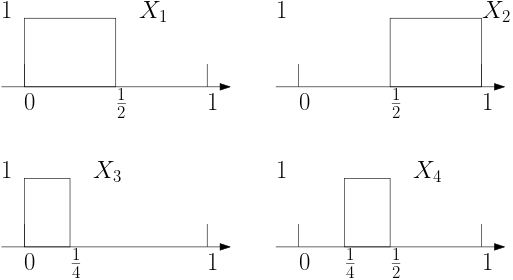
\includegraphics[width=.6\textwidth]{conv_prob} 
\caption{$X_n$ converges in probability but not almost surely.} 
\label{wk5:fg:Counter Example}
\end{figure}
\end{Example}

\section{Weak Law of Large Numbers}

Markov’s inequality: Suppose $a>0$ and $X\geq 0$. Then, 
\begin{align*}
a \indicatore{\{X\geq a\}}(\omega) \leq X\indicatore{\{X\geq a\}}(\omega)\leq X.
\end{align*}
Taking expectations, we have
\begin{align*}
a\P(X\geq a) & \leq \E X,\\
\P(X\geq a) & \leq \frac{1}{a}\E X.
\end{align*}

Chebyshev's inequality follows from Markov's inequality by replacing $X$ with $|X- \E X|^2$ and setting $a=\epsilon^2$: for $\epsilon>0$, 
\begin{align*}
\P( |X- \E X | \geq \epsilon) \leq \frac{1}{\epsilon ^2} \var(X).
\end{align*}

\begin{Theorem}[Weak Law of Large Numbers (WLLN)]\label{wk5:Thm:WLLN}
Suppose $X_1,X_2, \ldots$ are such that $\E X_i=0$, $\E X_i^2=\sigma^2<\infty$ and $\E[X_i X_j] \leq 0$ for  $i\neq j$. Then,
\begin{align*}
\ofrac{n} \sum_{i=1}^n {X_i} \convp 0 \text{ as } n \to \infty.
\end{align*}
\end{Theorem}
\begin{proof}
We have
\begin{align*}
\E[\left(\frac{1}{n} \sum_{i=1}^n{X_i}\right)^2] 
&= \frac{1}{n^2} \E [\sum_{i}^n{X_i^2}+2\sum_{i<j}{X_i X_j}]\\
& \leq \frac{1}{n^2}  \sum_{i}^n{\E X_i^2}= \frac{\sigma^2}{n}.
\end{align*}
From Chebyshev's inequality, we then have for any $\epsilon>0$, 
\begin{align*}
\P(\abs*{\frac{1}{n} \sum_{i=1}^n{X_i}} \geq \epsilon)\leq \frac{1}{\epsilon^2}\frac{\sigma^2}{n}\to 0,
\end{align*}
as $n\to\infty$.
\end{proof}


\section{Product Measures}

Given two measure spaces $(\Omega_1, \calA_1, \mu_1)$ and $(\Omega_2, \calA_2, \mu_2)$, where both $\mu_1$and $\mu_2$ are $\sigma$-finite, we can define a new measurable space $(\Omega, \calF)$, where $\Omega=\Omega_1\times\Omega_2$ and 
\begin{align*}
\calF= \sigma\left\{A \times B: A\in \calA_1, B\in \calA_2 \right\}.
\end{align*}
We call $A\times B$ a rectangle. A natural measure $\mu$ for this measurable space satisfies 
\begin{align}\label{prod_mu}
\mu (A \times B )=\mu_1 (A) \mu_2(B)
\end{align}
for all rectanges $A\times B$. It can be checked that the collection of finite disjoint unions of rectangles is an algebra (exercise). To extend this measure $\mu$ to $\calF$, we make use of Caratheodory's Extension Theorem (\cref{Caratheodory Theorem}): we show that for $A\times B = \bigcup_{i \geq 1} {A_i \times B_i}$ a disjoint union of rectangles, we have $\mu (A \times B)= \sum_{i \geq 1} {\mu_1 (A_i) \mu_2(B_i)}$. 

For $x \in A$, let $I(x)=\{i:x \in A_i\}$ and $B= \bigcup_{i \in I(x)} {B_i}$ a disjoint union. We have
\begin{align*}
\indicatore{A}(x) \mu_2(B) 
&=\indicatore{A}(x) \mu_2\left(\bigcup_{i \in I(x)} {B_i}\right)\\
&= \sum_{i \in I(x)} \indicatore{A}(x) \mu_2 (B_i)\\
& =\sum_{i\geq 1} \indicatore{A_i}(x) \mu_2 (B_i).
\end{align*}
Integrating w.r.t.\ $\mu_1$, we have
\begin{align*}
\mu (A\times B) 
%&= \mu_1(A) \mu_2(B)\\
&=\int \lim_{n \to \infty}{\sum_{i=1}^n {\indicatore{A_i} (x)\mu_2 (B_i) \ud \mu_1}}\\
&\stackrel{\text{MCT}}{=}\lim_{n \to \infty} \int {\sum_{i=1}^n {\indicatore{A_i} (x)\mu_2 (B_i) \ud \mu_1}}\\
& =\lim_{n \to \infty}\sum_{i=1}^n{\int  \indicatore{A_i} (x)\mu_2 (B_i) \ud \mu_1}\\
& =\sum_{i\geq 1}\mu_1(A_i)\mu_2 (B_i),
\end{align*}
where the interchange of the sum and integral in the penultimate equality holds because the number of terms is finite. Therefore, Caratheodory’s Extension Theorem shows that there is a unique extension of $\mu$ defined by \cref{prod_mu} to $\calF$. This is called a \emph{product measure}. Notationally, we write $\mu = \mu_1 \times \mu_2$.

The next theorem tells us when we can interchange integrals in general.
\begin{Theorem}[Fubini or Fubini-Tonelli]\label{wk5:Fubini_theorem}
Suppose $(\Omega_1, \calA_1, \mu_1)$ and $(\Omega_2, \calA_2, \mu_2)$ are $\sigma$-finite and $\mu = \mu_1 \times \mu_2$ is the product measure. Consider a measurable function $f:\Omega=\Omega_1\times\Omega_2 \mapsto \Real$. If $f \geq 0$ or $\int{|f|} \ud\mu< \infty$, then
\begin{align*}
\int_{\Omega_1} \int_{\Omega_2} f (x,y) \ud \mu_2 \ud \mu_1 = \int_{\Omega} f \ud \mu = \int_{\Omega_2} \int_{\Omega_1} f (x,y) \ud \mu_1 \ud \mu_2.
\end{align*}
\end{Theorem}
\begin{proof}
Note that implicit in the theorem statement are the following that we need to prove:
\begin{enumerate}[(i)]
\item For each $x \in \Omega_1$, $y \mapsto f(x,y)$ is $\calA_2$-measurable.
\item  $x \mapsto \int_{\Omega_2} f(x,y) \ud \mu_2$ is $\calA_1$-measurable.
\item $\int_{\Omega_1} \int_{\Omega_2} f (x,y) \ud \mu_2 \ud \mu_1 = \int_{\Omega} f \ud \mu$.
\end{enumerate}
Without loss of generality, we may assume $\mu_1,\mu_2<\infty$ as the same proof is valid on each partition of $\Omega$ and then we can apply the MCT.

The proof follows the steps discussed at the end of \cref{sec:Expectation}. We first prove the theorem for the simplest case where $f = \indicatore{E}$, where $E\in \calF$, the product $\sigma$-algebra. Let $E_x=\{y:(x,y)\in E\}$. 

(i): Fix $x$, then $y \mapsto f(x,y)= \indicatore{E_x}(y)$. We need to show $E_x \in \calA_2$. Let $\calE=\{E \in \calF : E_x \in \calA_2\}$. We have $(E^c)_x=(E_x)^c$ since $y \in (E^c)_x \Leftrightarrow (x,y)\in E^c \Leftrightarrow y\in (E_x)^c$, and $\left(\bigcup_{i\geq1} E_i\right)_x = \bigcup_{i\geq1} (E_i)_x$. Therefore, $\calE$ is a $\sigma$-algebra and it contains all rectangles $A \times B$ where $A\in \calA$ and $B\in \calB$, which implies that $\calF \subset \calE$.

(ii) $\&$ (iii): Let $\calL=\set*{E \in \calF\given f= \indicatore{E} \text{ satisfies (ii) \&(iii)}}$. 
\begin{itemize}
\item $\Omega \in \calL$.
\item  If $E \in \calL$, $\mu_2((E^c)_x) =\mu_2((E_x)^c)=\mu_2(\Omega_2)-\mu_2(E_x)$. Since $\mu_2(\Omega_2)< \infty$ and $\mu_2(E_x)$ is $\calA_1$-measurable, $\mu_2((E^c)_x)$ is $\calA_1$-measurable. We also have
\begin{align*}
\int \mu_2((E^c)_x) \ud \mu_1
& =\mu_2(\Omega_2)\mu_1(\Omega_1)-\int \mu_2(E_x) \ud \mu_1\\
& =\mu(\Omega)-\mu(E)\\
& =\mu(E^c).
\end{align*}
Therefore, $E^c \in \calL$.

\item If $E_i \in \calL$, $i\geq 1$, are disjoint, then
\begin{align*}
\mu_2\parens*{\parens{\bigcup_{i \geq 1}E_i}_x}
&=\mu_2\left(\bigcup_{i \geq 1}({E_i})_x\right) \\
& = \sum_{i \geq 1} \mu_2((E_i)_x)\\
& =\lim_{n \to \infty} \sum_{i=1}^n \mu_2((E_i)_x),
\end{align*}
which is $\calA_1$-measurable from \cref{lem:wk4:infX_rv} since each $\mu_2((E_i)_x)$ is $\calA_1$-measurable. From the MCT, we have
\begin{align*}
\int \mu_2\left((\bigcup_{i \geq 1}{E_i})_x\right) \ud \mu_1 
& = \lim_{n \to \infty}{\int \sum_{i = 1}^n{\mu_2 ((E_i)_x} )\ud \mu_1 }\\
& =  \lim_{n \to \infty}{\sum_{i = 1}^n{\int \mu_2 ((E_i)_x} )\ud \mu_1 }\\
& = \lim_{n \to \infty}\sum_{i=1}^n \mu (E_i)\\
& = \mu\parens*{\bigcup_{i \geq 1} {E_i}}.
\end{align*}
\end{itemize}
Therefore, $\calL$ is a $\lambda$-system containing the collection of rectangles, which is a $\pi$-system. From the $\pi$-$\lambda$ Theorem, we obtain $\calF \subset \calL$. We have now shown that Fubini's Theorem holds for $f=\indicatore{E}$, $E \in \calF$.

From linearity of integrals, the theorem holds for all simple functions $f$.

For $f \geq 0$, $\exists$ simple $f_i \uparrow f$. Applying MCT gives Fubini's theorem for non-negative $f$.

Finally, for general $f=f^+-f^-$, we note that $\int |f| \ud \mu <\infty$ implies $\int f^+ \ud \mu, \int f^- \ud \mu<\infty$, and
\begin{align*}
\int f^+ \ud \mu = \int \int f^+(x,y) \ud \mu_1 \ud \mu_2 \implies  \int f^+(x,y) \ud \mu_1 <\infty\ \text{$\mu_2$-a.e.} \\
= \int \int f^+(x,y) \ud \mu_2 \ud \mu_1 \implies  \int f^+(x,y) \ud \mu_2 <\infty\ \text{$\mu_1$-a.e.} 
\end{align*}
Similarly for $f^-$ so that
\begin{align*}
 \int \int f^+(x,y) \ud \mu_1 \ud \mu_2 - \int \int f^-(x,y) \ud \mu_1 \ud \mu_2 = \int \int f(x,y) \ud \mu_1 \ud \mu_2.
\end{align*}
The proof is now complete.
\end{proof}



\begin{Example}
\begin{equation}
\bordermatrix{
& x &&  \longrightarrow \cr
&\vdots && \vdots && \vdots&& \vdots \cr\\
&0\ && 0 && 0 \ && 1 && \ldots \cr\\
y \bigg\uparrow &0\ && 0 && 1 \ && -1 && \ldots \cr\\
&0\ && 1 && -1 \ && 0 && \ldots \cr\\
&1\ && -1 && 0 \ && 0 && \ldots \cr
}
\end{equation}
We have
\begin{align*}
\sum_y \sum_x f(x,y) &= \sum_y 0 = 0.\\
\sum_x \sum_y f(x,y) &= 1+0+0+\cdots = 1.
\end{align*}
This example shows that the conditions in Fubini's Theorem are essentially necessary. 
\end{Example}


\begin{Example}
Suppose $((0,1),\calB (0,1),\lambda) \times ((0,1),2^{(0,1)},\nu)$, where $\nu(A)=|A|$ is the counting measure, which is not $\sigma$-finite. Let
\begin{equation}
f(x,y)=\left\{
\begin{aligned}
1, && \text{if } x=y,\\
0, && \text{otherwise.} 
\end{aligned}
\right.
\end{equation}
Then we have
\begin{align*}
\int f(x,y) \ud \nu = 1 \text{ for each } x \implies \int \int f(x,y) \ud \nu \ud \lambda= 1,\\
\int f(x,y) \ud \lambda = 0 \text{ for each } y \implies \int \int f(x,y) \ud \lambda \ud \nu= 0.
\end{align*}
This example shows that $\sigma$-finiteness of the measures is necessary. 
\end{Example}




\section{Independence}

Throughout this section, we consider a probability space $(\Omega,\calA,\P)$.

\begin{Definition}
Two events $A$ and $B$ are independent if $\P(A \cap B) = \P(A)\P(B)$. We write $A \independent B$.
\end{Definition}

If $A \independent B$, then it is easy to verify the following:
\begin{enumerate}[(i)]
\item $A^c \independent B$.
\item $A \independent B^c$.
\item $A^c \independent B^c$.
\end{enumerate}
I.e., the two $\sigma$-algebras $\{\emptyset,\Omega ,A, A^c\}$ and $\{\emptyset,\Omega ,B, B^c\}$ are ``independent''.

\begin{Definition}
The sub-$\sigma$-algebra $\calA_i \subset \calA$, $i=1,2,\ldots, n$, are independent if $\forall A_i \in \calA_i$, 
\begin{align*}
\P(\bigcap_{i=1}^n {A_i})= \prod_{i=1}^n {\P(A_i)}.
\end{align*}
They are said to be \emph{pairwise independent} if $\P(A_i \cap A_j)=\P(A_i)\P(A_j)$ $\forall i \neq j$.
\end{Definition}

We say that the random variables $X_1,X_2,\ldots,X_n$ are independent if $\sigma(X_i)$, $i=1,\ldots,n$, are independent, i.e., $\forall B_i \in \calB$, $i=1,\ldots,n$,
\begin{align*}
\P (X_1\in B_1,X_2\in B_2,\ldots,X_n\in B_n)= \prod_{i=1}^n {\P(X_i \in B_i)}.
\end{align*}

Note that independence $\implies$ pairwise independence but the converse is false. Here are two counter examples to show that pairwise independence does not imply independence.

\begin{Example}\label{wk5:Independence1}
\begin{figure}[!htb]
\centering
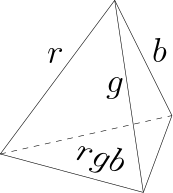
\includegraphics[width=.2\textwidth]{wk5_tetrahedron.png} 
\caption{Dice example: pairwise independence does not imply independence.} 
\label{wk5:fg:Independence}
\end{figure}
Consider a fair tetrahedron dice that has one red edge, one green edge and one blue edge as shown in \cref{wk5:fg:Independence}. The bottom has all three colors. Let $r$ be the event that the dice when tossed lands on a face with a red boundary. The events $b$, $g$ and $rgb$ are defined similarly. Then, by symmetry, we have
\begin{align*}
&\P (r)=\P(g)=\P(b)=\frac{1}{2}, \\
&\P (rgb)=\P(rg)=\P(gb)=\P(rb)=\frac{1}{4}.
\end{align*}
Therefore, these events are pairwise independent but not independent.
\end{Example}

\begin{Example}\label{wk5:Independence2}
Consider two six-sided fair dice. Let
\begin{align*}
A_1 & =\{ \text{1st dice is odd} \}, \\
A_2 & =\{ \text{2nd dice is odd} \},\\
A_{sum} & =\{ \text{sum of the two dice is odd} \}.
\end{align*}
We have
\begin{align*}
&\P (A_1) =\P (A_1) =\P (A_{sum}) =\frac{1}{2},\\
&\P (A_1\cap A_2) =\P (A_1\cap A_{sum})=\P (A_2\cap A_{sum}) =\frac{1}{4},\\
&\P (A_1\cap A_2 \cap A_{sum}) =0.
\end{align*}
Therefore, the events are pairwise independent but not independent. In particular, $\sigma(A_1)$ is not independent with $\sigma(\{A_2,A_{sum}\})$.
\end{Example}

\begin{Lemma}\label{wk5:lem:pi-independent} 
Suppose the two collections of subsets $\calE$ and $\calC$ are $\pi$-systems and $\P(B \cap C)=\P(B) \P (C),\ \forall B \in \calE$, $C \in \calC$. Then $\sigma (\calE)$ and $\sigma (\calC)$ are independent.
\end{Lemma}
\begin{proof}
Let $\calD_1=\{D \in \calA : \P (D\cap C)= \P(D) \P(C), \forall C \in \calC \}$. As an exercise, one can check that $\calD_1$ is a $\lambda$-system. Since $\calE \subset \calD_1$, from the $\pi$-$\lambda$ theorem we have $\sigma(\calE)\subset \calD_1$.

Let $\calD_2=\{D \in \calA : \P (B\cap D)= \P(B) \P(D), \forall B \in \sigma(\calE) \}$. Similarly $\calD_2$ is a $\lambda$-system. From above, $\calC \subset \calD_2$ and by the $\pi$-$\lambda$ theorem, we have $\sigma(\calC)\subset \calD_2$. Therefore, $\sigma (\calE) \independent \sigma (\calC)$.
\end{proof}
By induction, if $\calB_i$ for $i=1,\ldots,n$ are $\pi$-systems and are independent, then $\sigma(\calB _i)$ are independent.

\begin{Corollary}
The random variables $X_1,X_2,\ldots,X_n$ are independent if 
\begin{align*}
\P (X_1\leq t_1,X_2\leq t_2,\ldots, X_n\leq t_n)= \prod_{i=1}^n {\P(X_i\leq t_i)}.
\end{align*}
\end{Corollary}
\begin{proof}
Since $\{(-\infty,t]: t\in\Real\}$ is a $\pi$-system that generates $\calB(\Real)$, the corollary follows from \cref{wk5:lem:pi-independent}.
\end{proof}

\begin{Lemma} 
Suppose that each random variable $X_i$ has pdf $f_i$, $i=1,\ldots,n$. Then $X_1,\ldots , X_n$ are independent iff $\exists$ a joint pdf $f(x_1,\ldots,x_n)=\prod_{i=1}^n {f_i (X_i)}$.
\end{Lemma}
\begin{proof}
`$\Leftarrow$':
\begin{align*}
\P (\bigcap_{i=1}^n \{X_i \in A_i\}) & = \int_{A_1 \times \cdots \times A_n} f(x_1, \ldots, x_n) \ud x_1 \cdots \ud x_n\\
& = \int_{A_1 \times \cdots \times A_n} \prod_{i=1}^n {f(x_i)} \ud x_1 \cdots \ud x_n\\
& =  \prod_{i=1}^n \int_{A_i} {f(x_i)} \ud x_i\\
& =  \prod_{i=1}^n {\P (X_i \in A_i)}. 
\end{align*}
`$\Rightarrow$':
Let $X=(X_1,\ldots,X_n)$. For $A_i \in \calB$, $i=1, \ldots n$, we are given
\begin{align}
\P(X \in A_1\times \cdots \times A_n) & =\prod_{i=1}^n {\P (X_i \in A_i)}\nn
& =  \prod_{i=1}^n \int_{A_i} {f_i(x_i)} \ud x_i\nn
& = \int_{A_1 \times \cdots \times A_n} \prod_{i=1}^n f_i(x_i) \ud x_1\cdots\ud x_n.\label{prodA}
\end{align}
We want to show that 
\begin{align*}
\P(X\in A) = \int_A \prod_{i=1}^n f_i(x_i) \ud x_1\cdots\ud x_n
\end{align*}
for all $A$ in the product $\sigma$-algebra $\calB(\Real^n)=\sigma \{A_1 \times \cdots \times A_n: A_i \in \calB\}$. 

Let $\calL=\{A \in \calE : \P(X\in A)= \int_{A} \prod_{i=1}^n {f_i(x_i)} \ud x_1 \cdots \ud x_n\}$. It can be checked that $\calL$ is a $\lambda$-system and $\calP = \{ {A_1 \times \cdots \times A_n}: A_i \subset \calB\}$ is a $\pi$-system and generates $\calB(\Real^n)$. Since $\calP \subset \calL$ from \cref{prodA}, by the $\pi$-$\lambda$ Theorem, we have $\sigma(\calP) \subset \calL$ and the proof is complete.
\end{proof}

\begin{Lemma}
If $X \independent Y$ and are integrable, then $\E[XY]=\E X \E Y$.
\end{Lemma}
\begin{proof}
The distribution of $(X,Y)$ on $\Real^2$ is the product measure $\P_X \times \P_Y$. From Fubini's theorem, we have
\begin{align*}
\E[XY] = \int_{\Real^2} xy \ud \P_X\times\P_Y(x,y) = \int_\Real x \ud\P_X(x) \int_\Real y \ud \P_Y(y) = \E X \E Y.
\end{align*}
\end{proof}

Suppose $X \independent Y$. For any measurable functions $f$ and $g$, $f(X)\independent g(Y)$ since $\sigma(f(X)) \subset \sigma(X)$.



%\bibliography{mybib}
\bibliographystyle{alpha}

\end{document}
